\section{Motivation}
\label{sec:Motivation}

Typical web applications experience large variations in user traffic over
time.\footnote{Roy \etal~\citep{Roy:2015:ISN:2785956.2787472} and Bronson
\etal~\citep{180185} show network bytes over the course of the day for a web-server and
memcached~\citep{Nishtala2013ScalingFacebook} at Facebook.}
Figure~\ref{fig:websearchmotivation}, for example, shows how the number of queries per second during a web search, 
a typical load at Google data centre, varies between about
\SI{5}{\percent} and \SI{80}{\percent} of maximum capacity~\citep{Hoelzle2009TheMachinesb,
Meisner2011PowerServices,Lo2014TowardsWorkloads}.  Similarly, Facebook consistently sees
diurnal load variations between \SI{10}{\percent} and \SI{95}{\percent} of maximum
capacity, across multiple server clusters~\citep{Bilgir_exploringthe,
Atikoglu2012WorkloadStore}.

\begin{figure}[ht]
	\centering
    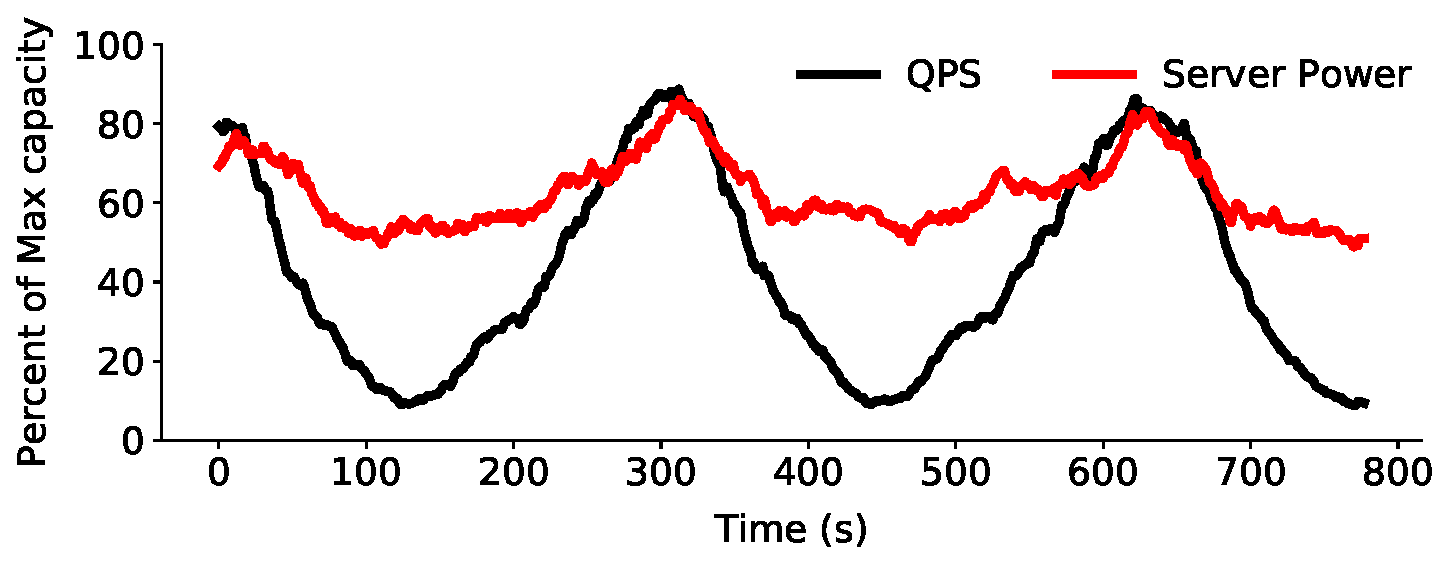
\includegraphics[width=\textwidth]{Chapter4/Figs/google_trace.eps}
    \caption[Power drawn for a diurnal load]{\captitle{Power drawn for a diurnal load~\citep{Meisner2011PowerServices,Lo2014TowardsWorkloads,Hoelzle2009TheMachinesb}.} The power consumption is measured for Web-Search running on two big cores of the ARM Juno R1 (64-bit big.LITTLE) platform.}
	\label{fig:websearchmotivation}
\end{figure}


The periods of low server utilisation provide opportunity to reduce data centre energy
consumption~\citep{Petrucci2015Octopus-Man:Computers, Lo2015Heracles,
Delimitrou2013Paragon:Datacenters, Delimitrou:2013:QSH:2542150.2556583}. As seen in
Figure~\ref{fig:websearchmotivation}, although load drops dramatically, power consumption
is always at \SI{60}{\percent} or above.  For this reason, both academia and industry are
working towards better energy proportionality; i.e. that the system's power consumption is
proportional to utilisation.

There are also opportunities to improve energy efficiency using heterogeneous servers
combined with DVFS. Heterogeneous servers can minimise power consumption at low load by
deploying small cores, and can provide maximum performance using big cores to meet the QoS
target for latency-critical workloads~\citep{Petrucci2015Octopus-Man:Computers,
JanapaReddi2010WebCores, Chitlur2012QuickIA:Prototypes}.

\paragraph{Mixing different core types with DVFS.} Figure~\ref{fig:octomancomp} shows the
energy efficiency in RPS/Watt and QPS/Watt when using a state-of-the-art baseline
policy~\citep{Petrucci2015Octopus-Man:Computers}.\footnote{Recall, RPS refers to requests
per second and QPS refers queries per second (see section~\ref{sec: perfmon thesis})} We
explore a heterogeneous architecture mixing different core types and DVFS (HetCMP) 

\begin{figure}[htbp]
\begin{subfigure}{\textwidth}
  \centering
  \includegraphics[width=0.9\linewidth]{Chapter4/Figs/rps-watt-memcached.eps}
  \caption{Memcached}
  \label{fig: improvements}
\end{subfigure}
%\hspace{-2.8em}
\begin{subfigure}{\textwidth}\ContinuedFloat
  \centering
  \includegraphics[width=0.9\linewidth]{Chapter4/Figs/rps-watt-websearch-new.eps}
  \caption{Web-Search}
  \label{fig: improvements-websearch}
\end{subfigure}
\begin{subfigure}{\textwidth}\ContinuedFloat
  \centering
  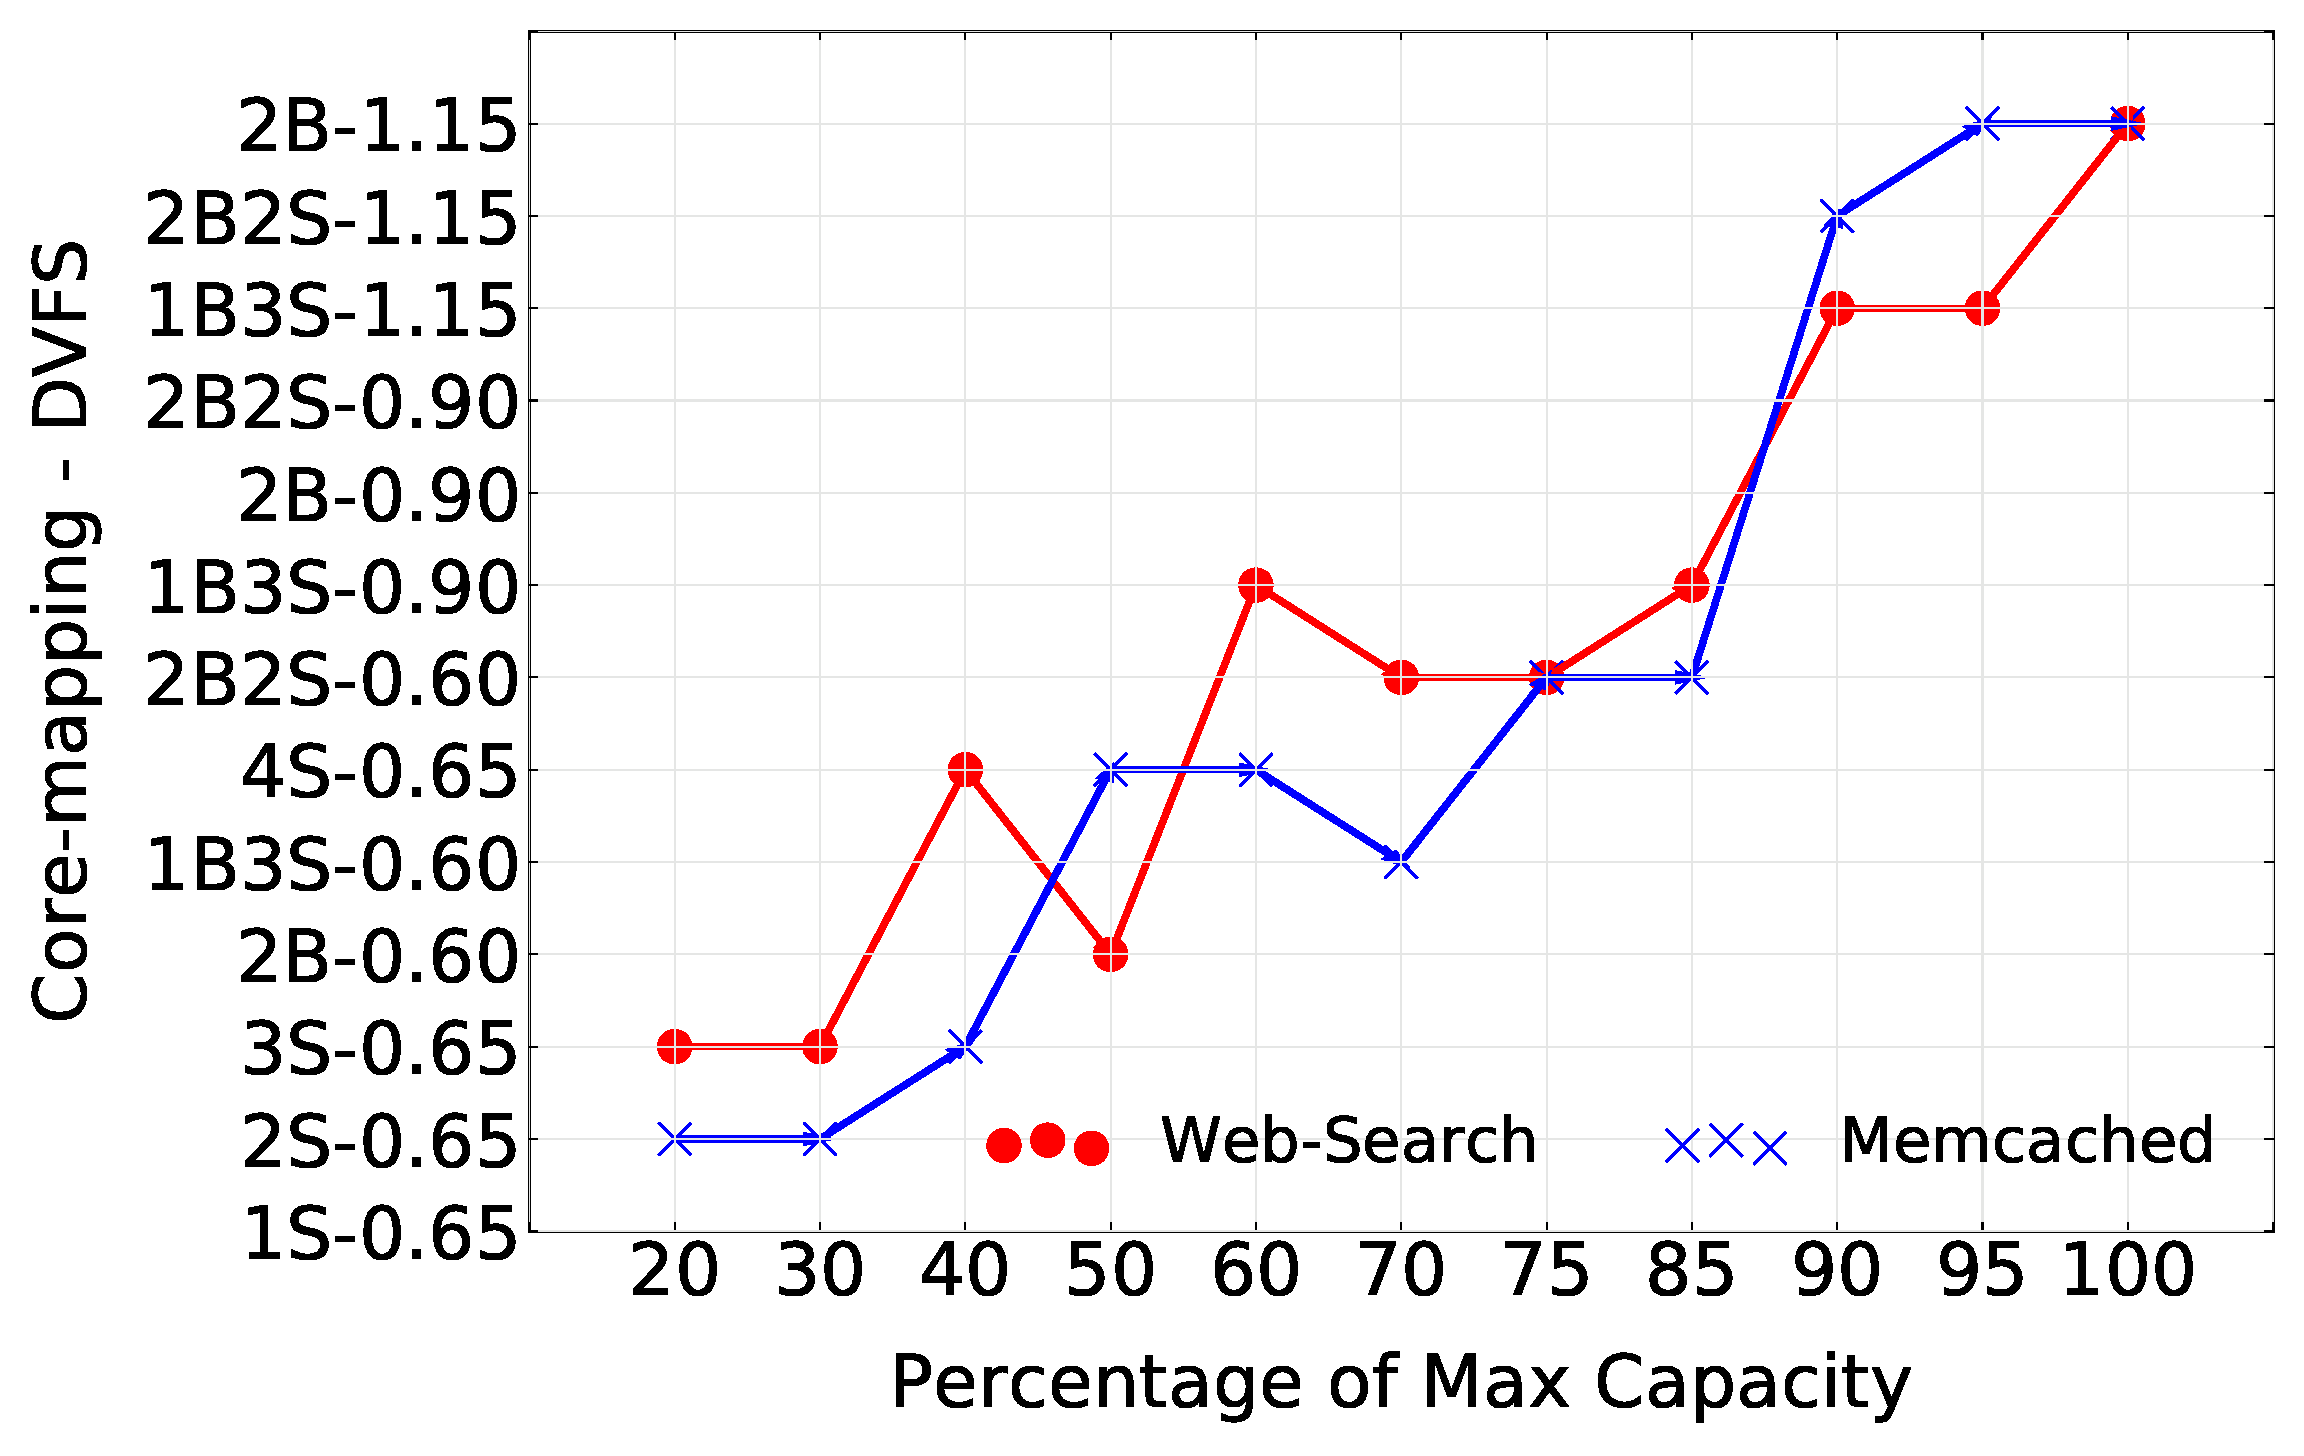
\includegraphics[width=0.9\linewidth]{Chapter4/Figs/state-transition.eps}
  \caption{State Machine}
  \label{fig: state-transition}
\end{subfigure}
    \caption[Throughput per watt of baseline policy vs heterogeneous platform with DVFS]{\captitle{Throughput per watt of baseline policy (BP)~\citep{Petrucci2015Octopus-Man:Computers} vs heterogeneous platform with DVFS (HetCMP).} Throughput per watt of Memcached (\ref{fig: improvements}) and Web-Search (\ref{fig: improvements-websearch}) with BP and HetCMP at different load levels along with their respective state machines (\ref{fig: state-transition})}
\label{fig:octomancomp}
\end{figure}

\noindent running Memcached (Figure~\ref{fig: improvements}) and Web-Search
(Figure~\ref{fig: improvements-websearch}) at different load levels. For each policy,
among the configurations where the QoS is met at each load level, the configuration with
the least power consumption is selected.  The table at the bottom of each subfigure shows
the configuration selected by HetCMP and our baseline policy. In the configurations of the
embedded table, $B$ and $S$ represent big and small cores, respectively. The configuration
space for HetCMP consists of core-mappings (big and small cores) and DVFS combinations for
a heterogeneous platform, whereas the baseline policy consists exclusively of either big
or small cores at the highest DVFS. The configurations available for the baseline policy
are therefore a subset of HetCMP. Experimental details of the ARM platform are given in
Chapter~\ref{chap: infrastructure}.



Figure~\ref{fig:octomancomp} raises two main concerns with current state-of-the-art
heuristic algorithm~\citep{Petrucci2015Octopus-Man:Computers}. First, Figure~\ref{fig:
improvements} demonstrates in periods of low load (less than \SI{60}{\percent} of max
capacity for Memcached), exclusive use of low performance cores at lower DVFS ensures QoS
is met while reducing static-power, thus making it an excellent option to use for periods
of low load. As the load increases, HetCMP transitions from low performance cores to a
best combination of small and big cores at a given DVFS (for instance, 2 big and 2 small
cores -- 2B2S at \SI{0.9}{\giga\hertz} at \SI{89}{\percent} load) to deliver the required
latency.  On the other hand, the baseline policy transitions directly from low performance
cores to high performance cores at highest DVFS to deliver the required latency, thereby
increasing energy consumption by \SI{27.74}{\percent} (mean). In periods of very high load
(more than \SI{90}{\percent} for Memcached), exclusive use of high performance cores at
higher DVFS ensures QoS is met with better energy proportionality.  Similarly results were
observed for Web-Search (Figure~\ref{fig: improvements-websearch}) with up to
\SI{25}{\percent} (mean) energy savings. The state-machine configuration for Memcached and
Web-Search are represented by the blue and red line, respectively, in Figure~\ref{fig:
state-transition}.

In summary, we show that small and big cores are an attractive option for periods of low
load and very high load, respectively, while meeting QoS targets at a much lower cost. On
the other hand, for intermediate loads, which are generally experienced by data centres
during the day~\citep{Vamanan2015TimeTrader:Search}, harnessing HetCMP provides the
opportunity for higher performance at a lower cost.


\paragraph{Exploring workload particularities.} We note that prior
work~\citep{Petrucci2015Octopus-Man:Computers} relies on a general single heuristic to
allocate exclusively big or small cores to workloads. By allowing an arbitrary allocation
mix of big and small cores with DVFS, this kind of heuristic can be sub-optimal across
diverse applications and architectures (evaluation details in Section~\ref{sec:
evaluation-hipster}); that is, a single state-machine management (as used in prior work)
may fail to precisely satisfy the QoS targets given distinct workload characteristics of
diverse applications. To illustrate this point, Figure~\ref{fig: state-transition} shows
two distinct/unique state transition mappings that are optimal (throughput per watt) at
different load capacities for Memcached and Web-Search.

\begin{figure}[t!]
    \centering
    \includegraphics[width=\textwidth]{Chapter4/Figs/config_exchange_new.eps}
    \caption[Energy efficiency of Memcached and Web-Search with state-machines exchanged.]{\captitle{Energy efficiency of Memcached and Web-Search with state-machines exchanged.} Energy efficiency at various load levels for Memcached while meeting QoS, using the state-machine of Web-Search normalised to the state-machine of Memcached (\textit{lower is worse}); converse for Web-Search.}
    \label{fig:config-exchange}
\end{figure}

Figure~\ref{fig:config-exchange} shows the energy efficiency that would be neglected
(ensuring QoS is met at different load levels) when using the state-machine built for
Web-Search but used for the manage the Memcached workload, normalised to the energy
efficiency using the state-machine built exclusively for Memcached; and vice-versa. The
state-machine configuration for Memcached and Web-Search are represented in blue and red
line, respectively, in Figure~\ref{fig: state-transition}.
Figure~\ref{fig:config-exchange} demonstrates that different latency-critical applications
benefit from different state-transition mappings and show improvement in energy efficiency
up to \SI{35}{\percent} for Memcached (at \SI{90}{\percent} load) and up to
\SI{19}{\percent} for Web-Search (at \SI{50}{\percent} load).  For instance, at low loads
and at very high loads both applications use exclusively small cores (low static power) or
big cores (high static power), respectively.  However, for intermediate loads, the
configurations in the state-transition for Web-Search are not present in Memcached and
vice-versa, thus providing minimal to no energy optimisation.

In practical scenarios, each workload has a time-varying load~\citep{Li2014TalesTail} and
a QoS target that needs to be met. As shown in Figure~\ref{fig:octomancomp}
and~\ref{fig:config-exchange}, there exists a unique configuration for each load  that
optimises energy efficiency. Moreover, the time-varying load presented in two forms:
sudden load spikes~\citep{Dean2013TheScale} or gradual load
changes~\citep{Meisner2011PowerServices, Hoelzle2009TheMachinesb}. Both these forms
present a challenge for a heuristic based approach as it jumps across multiple
configurations to meet the QoS target, thereby leading to QoS violations due to rampant
core oscillations.  Also, Kasture \etal~\citep{Kasture2015Rubik} note that
core-transitions are far more costly -- relative to DVFS changes.

There is a need for application agnostic learning approach that can exploit the energy
efficiency benefits of heterogeneous architectures and DVFS features, and can deal with
sudden/gradual load changes across different levels. This is precisely what
\textbf{Hipster} delivers.

